\documentclass[11pt,a4paper]{article}
\usepackage[ngerman]{babel}							% enables Hyphenation for german
% \usepackage[babel, german=quotes]{csquotes}
\usepackage{subfigure}								% enables subfigures
\usepackage{amsmath}								% enhances math output
\usepackage{amsfonts}								% additional math fonts
\usepackage{graphicx}								% alternativ graphic interface
\usepackage{color,listings}	 						% codesequences 
\usepackage{import}
\usepackage{cite}
\usepackage{enumitem}
%löst Probleme mit ä,ö,ü
\usepackage[utf8]{inputenc}
%\usepackage[T1]{fontenc}
%Deutsche Silbentrennung
\usepackage[ngerman]{babel}
% \usepackage{biblatex}
\usepackage{fancyhdr}			%% fuer Pagestyle fancyhdr mit eigenen Kopf und Fusszeilen

\setlength{\parindent}{0pt}		% to avoid american style paragraph indention (Einrücken)

\author{Heinz Hofmann und Jonas Schmid}

%% Pagestyle mit eigenen Kopf und Fusszeilen
\pagestyle{fancy}
\fancyhf{}								%% leerraeumen
% \fancyhead[L]{\includegraphics[height = 20pt]{logo.png}}
% \fancyhead[R]{Simulationstools}
\renewcommand{\headrulewidth}{0.0pt}	%% obere Trennlinie
\fancyfoot[L]{H. Hofmann und J. Schmid}
\fancyfoot[C]{\thepage}					%% Seitennummer
\fancyfoot[R]{20. Dezember 2017}		
\renewcommand{\footrulewidth}{0.4pt}	%% untere Trennlinie


\begin{document}

\section*{ \center \textbf{\LARGE Algorand: Eine vielversprechende Blockchain basierte Kryptow\"ahrungen}}
% \center \textbf{\LARGE Algorand: Eine vielversprechende Blockchain basierte Kryptow\"ahrungen} \\

Die populärsten Blockchain basierten Kryptow\"ahrungen wie Bitcoin und Ethereum haben noch einige technische M\"angel.
Insbesondere der Energie verschwenderischen Proof-of-Work kann auch wegen den grossen
und damit m\"achtigen Mining Pools zum Problem werden.
Zudem stossen Bitcoin und in absehbarer Zeit auch Ethereum an ihre Kapazit\"atsgrenzen (Transaktionen pro Zeit).
Einige Leute um den MIT Professor und Turing Award Winner Silvio Micali haben die alternative Cryptow\"ahrung Algorand entwickelt.
Diese soll eine deutlich gr\"ossere Kapazit\"at bereitstellen als bisherige Blockchain basierte L\"osungen und anstelle von Proof-of-Work wird ein Proof-of-Stake Verfahren angewandt.
Algorand befindet sich im Entwicklungsstadium und wird noch nicht in der Praxis eingesetzt.
Die Offenen Punkte und Probleme welche Algorand aufweist sind im Paper gut beschrieben.
Es wurde jedoch erfolgreich ein Prototyp mit einigen hunderttausend Nodes simuliert\cite[Kapitel Implementation \& Evaluation]{Gilad:2017:ASB:3132747.3132757}.
Dabei wird eine \grqq{}Transaction Confirmation Time\grqq{} von rund einer Minute erreicht und es k\"onnen rund 125 mal mehr Transaktionen get\"atigt werden als bei Bitcoin.
Nachfolgend beziehen wir uns mehrheitlich auf das Paper \cite{Gilad:2017:ASB:3132747.3132757},
welches Algorand resp. den Algorithmus detailliert und unserer Meinung nach sehr gut beschreibt.
Alternativ beschreibt das Paper \cite{Chen:2017} den Algorithmus,
ein grober \"Uberblick verschafft der Beitrag \cite{ScalingConsensus},
darin wird vor allem die Skalierbarkeit des Byzantine Agreement Algorithmus betont.

\section*{\"Ubersicht}
Algorand basiert auf einer Blockchain sehr \"ahnlich wie Bitcoin.
Um Konsens bez\"uglich des jeweilig n\"achsten Blockes zu erreichen,
wird der n\"achste Block resp. der jeweilige Erzeuger mittels Byzantine Agreement ermittelt.
Ein komplettes Byzantine Agreement mit allen Nodes ist jedoch wegen des viel zu hohen Kommunikationsaufwandes nicht durchf\"uhrbar.
Deshalb agiert bez\"uglich Byzantine Agreement immer nur ein Subset von Nodes\footnote{Beim Algorand Prototypen wurden 26 Nodes angestrebt.}.
F\"ur jede Kommunikationsrunde werden die Rollen mittels \textit{cryptographic sortition} verteilt.


\newpage
% \chapter{\textbf{\Large Block zur Blockchain hinzuf\"ugen }}\\
\section*{N\"achsten Block ermitteln}
Das Hinzuf\"ugen eines Blocks zur Blockchain vollzieht sich in drei Steps. %, siehe auch Abbildung \ref{fig:algorand}.
\begin{enumerate}[label=\arabic*)]
	\item \textbf{Block erzeugen und broadcasten}\\
	Jeder Node f\"uhrt bei sich die Sortition durch, um herauszufinden, ob er einen Block broadcasten darf.
Falls ja, stellt dieser einen Block zusammen und \grqq{}broadcasted\grqq{} diesen im Netzwerk.
% Falls ja, f\"ugt er alle Transaktionen, die er m\"ochte dem Block hinzu und "broadcasted" diesen dem Netzwerk.
Er wird einer von ca. 26 Nodes sein, der einen Block broadcasten darf.
Jeder dieser ca. 26 gebroadcasteten Bl\"ocke hat aber eine gewisse Priorit\"at, welche ebenfalls durch die Sortition erzeugt wurde.
	 
	\item \textbf{Byzantine Agreement}\\
	Nun wird in zwei Substeps das Problem \grqq{}einen aus vielen Bl\"ocken ausw\"ahlen\grqq{} auf das bin\"are Problem \grqq{}entweder den gebroadcasteten Block oder einen leeren Block auszuw\"ahlen\grqq{} reduziert.
	\begin{enumerate}[label=\Roman*)]
		\item Nach einer bestimmten Wartezeit (zur Synchronisation) gibt ein Gremium - im Paper \textit{comittee} genannt - von zuf\"allig durch Sortition ausgew\"ahlten Nodes eine Stimme f\"ur je einen Block ab. Sie w\"ahlen jeweils von den f\"ur sie sichtbaren Blocks, denjenigen mit der h\"ochsten Priorit\"at.
		Diese Stimme broadcasten Sie wieder durch das Netzwerk.
		
		\item Ein erneut durch Sortition zuf\"allig gew\"ahltes Gremium wartet bis, entweder gen\"ugend Votes f\"ur einen Block zusammen gekommen sind, oder bis eine bestimmte Zeit abgelaufen ist.
		Sind gen\"ugend Votes zusammengekommen, wird der entsprechend gew\"ahlte Block promotet.
		Ist die Zeit abgelaufen, ohne dass gen\"ugend Votes zusammen gekommen sind, wird ein leerer Block promoted.
		Alle gutartigen Nodes werden hier entweder denselben vollen Block oder einen leeren Block promoten.
	\end{enumerate}
	\item \textbf{Binary Byzantine Agreement}\\
	Ab hier wird mittels Binary Byzantine Agreement zwischen dem zuvor ausgew\"ahlte Block oder einem leeren Block entschieden.
	Falls es keine fehlbaren Nodes gibt, ist dieser Prozess in zwei Substeps beendet.
	Wird der Prozess aber von fehlbaren Nodes gezielt durch Broadcasts von unterschiedlichen Bl\"ocken gest\"ort,
	kann dieser Vorgang bis zu 9 Substeps andauern.
	In jedem Substep wird jeweils ein neues Gremium gew\"ahlt,
	welches Votes f\"ur den zuvor ausgew\"ahlten oder einen leeren Block abgibt.
	In jedem Dritten Substep wird ausserdem eine \grqq{}gemeinsame\grqq{} M\"unze geworfen,
	dies hilft dem Prozess fort zu schreiten.
\end{enumerate}
% Der ganze Prozess dauert ca. 20 Sekunden. Konservativer weise wurden die Wartezeiten der Nodes, bis diese voten, so gew\"ahlt, dass der ganze Prozess rund eine Minute dauert.
Dieser ganze Prozess k\"onnte in rund 20 Sekunden abgewickelt werden.
Konservativer weise wurden die Wartezeiten so gew\"ahlt, dass es rund eine Minute dauert bis ein Block bestimmt wurde.

% \begin{figure}
% 	\centering
% 	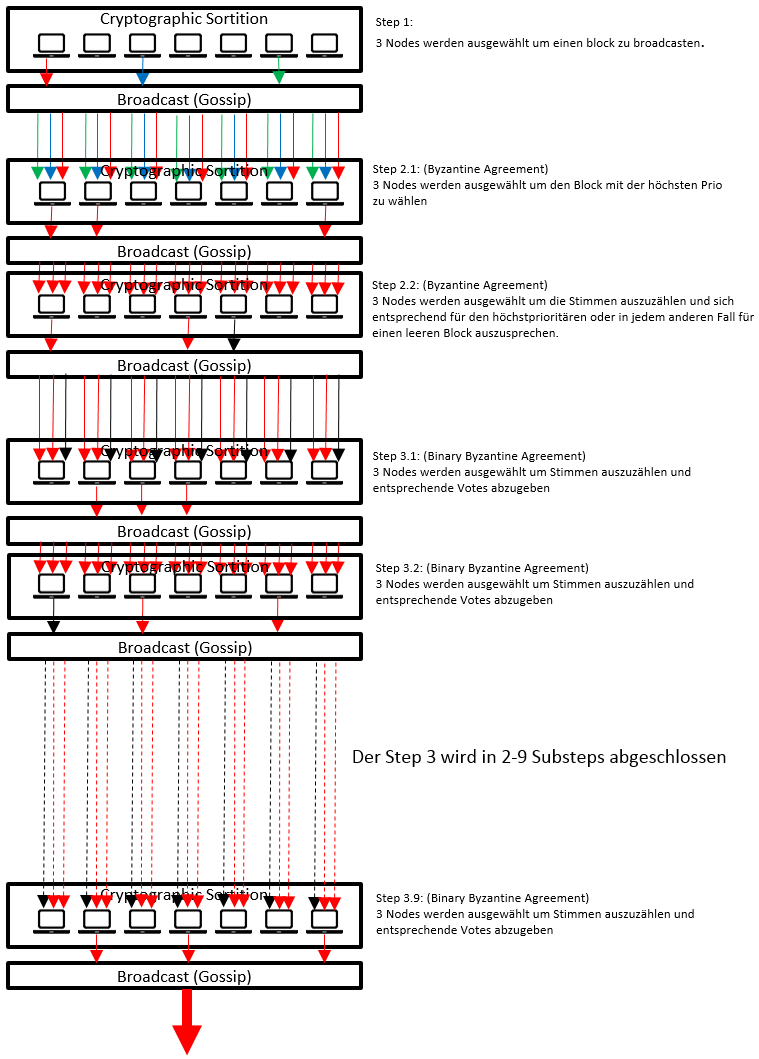
\includegraphics[scale=0.65]{Algorand.png}
% 	\caption{Kommunikationsablauf beim w\"ahlen resp. hinzufügen eines neuen Blockes.}
% 	\label{fig:algorand}
% \end{figure}


\section*{Cryptographic Sortition}
% \chapter{\textbf{\Large Cryptographic Sortition}}\\
F\"ur jede Kommunikationsrunde berechnet jeder Node f\"ur sich ob er f\"ur ein oder mehrere Mandate (Block broadcasten oder Gremium) gew\"ahlt ist.
Dazu wird mittels \textit{verifiable random function}, kurz VRF, aus dem \textit{private key} und einem bekannten \textit{seed} ein \textit{hash} und ein Beweis berechnet. % im Paper oft mit $\pi$ abgekürzt
Die Mandate werden abh\"angig vom jeweiligen Balance und berechnetem Hash der Nodes verteilt.
Das heisst ein Node welcher viel Geld im System hat, bekommt \"ofter ein Mandat zugeteilt als ein Node, welcher wenig Geld im System hat.
Somit ist das Auswahlverfahren vom Typ Proof-of-Stake und sch\"utzt Algorand vor \textit{Sybill attacks}.
Zudem ist so die Rolle der Miner und Kontoinhaber nicht trennbar, wie dies bei Bitcoin der Fall ist und zu Problemen f\"uhren kann.
Der \textit{seed} ist jeweils abh\"angig von den vorangehenden Kommunikationsrunde.
Weiter wird mit dem Hash jedem Node eine Priorit\"at zugeteilt, welche f\"ur das Byzantine Agreement verwendet wird.
Die VRF ist so konzipiert, dass der Hash nur mittels Private Key berechnet werden kann.
Somit kennt keiner die ausgew\"ahlten Nodes, bevor diese eine Mitteilung ins Netzwerk versendet und
damit ihr Mandat ausgef\"uhrt haben.
Damit ist ein Agriff auf nur diese wenigen Nodes nicht m\"oglich.
Mit dem Beweis aus der VRF und dem jeweiligen Public Key kann jeder Node jeden Hash und damit die Rollenzuteilung jedes Nodes \"uberpr\"ufen.

\section*{Fazit}
Algorand bedient sich einigen Verfahren aus der Kryptographie und Netzwerktheorie
und stellt damit ein elegantes und leistungsf\"ahiges Framework für ein Blockchain zur Verf\"ugung.
Jedoch ist es noch nicht ausgereift und muss sich erst noch in der realen Welt behaupten.
Ein Vergleich mit Bitcoin oder Ethereum ist daher nur sehr eingeschr\"ankt m\"oglich.
Interessanter wird der Vergleich, wenn Ethereum die Umstellung auf Proof-of-Stake vollzogen hat.
Die zur Verf\"ugung stehenden Quellen sind zudem noch auf nur einige wenige Leute am MIT oder der Stony Brook University zur\"uckzuf\"uhren. % Computer Science and Artificial Inteligence Laboratory


Das Paper \cite{Gilad:2017:ASB:3132747.3132757} w\"urde sich aber sicherlich gut eignen f\"ur weitere \grqq{}Diskussionrunden\grqq{}.
Es werden zudem einige Aspekte bez\"uglich Distributed Systems aufgegriffen welche
im Buch \grqq{}Distributed Ledger Systems\grqq{} von Roger Wattenhofer thematisiert wurden.


% \bibliographystyle{plain}
\newpage
\bibliographystyle{apalike} % makes reference labels like [Redmond et al., 2016]
\bibliography{algorand}{}

% \cite{Gilad:2017:ASB:3132747.3132757}


\end{document}
